\chapter{Case data: Population projection}\label{CCaseData}
The population projection visualized in this project have been created by \citet{Kessler} using a geosimulation, which geographically distribute a predicted population. This geosimulation has been run every tenth year from 2010 to 2100. It has also been run for different scenarios for the future.

\section{The data behind the simulation}\label{TheDataBehind}
This projection is a geographical distribution of the global prospects created by The United Nations Department of Economic and Social Affairs. These prospects estimate the population numbers in each country living in rural and urban areas. The spatial distribution has been based on raster data from the Global Rural Urban Mapping Project (GRUMP). In this dataset the world has been divided into 1x1 km cells, each of which contains the number of estimated people. \citep{Kessler}

The geosimulation has been run with two different definitions for the urban extent. The first one is also created by GRUMP. This urban extent has been estimated based on the light emitted after dark. It is known to overestimates the extent of urban areas. \citep{Kessler}
The second dataset was provided by Global Land Cover Map from the European Space Agency (GlobCover), where areas classified as “artificial surfaces and associated urban areas” in the GlobCover data were treated as urban areas. 

\section{The simulation}
Using this dataset to define the extent of urban and rural areas, the simulation was run as illustrated in figure \ref{CreatingData}.

\begin{figure} [H]
	\centering
	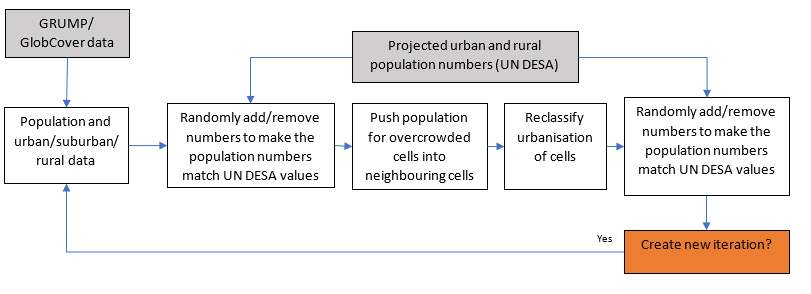
\includegraphics[width=1\textwidth]{Pictures/CreatingData}
	\caption{A flowdiagram of simulation creating the population projections}
	\label{CreatingData}
\end{figure}

The population in rural and urban areas were adjusted to match the projected values from UN DESA. This was done by randomly adding or removing people from the area types. 

The cells would have a country-specific limit on how many people could live in them. Any cells with a population above this limit would push the excess population to neighboring cells. 

After this, the cells would be reclassified as more urbanized if their population had increased above a country-determined threshold. This way a rural cell might become a suburban one or a suburban become urban if its population increased. The data is then adjusted to match projected values again with the same approach as before. This is required because the reclassification would mean that the number for the different urbanization classes would no longer match the numbers from UN DESA.

These steps are then repeated for every iteration. 

\citep{Kessler}
\section{Shared Socioeconomic Pathways} \label{SSPs}

\begin{figure} [H]
	\centering
	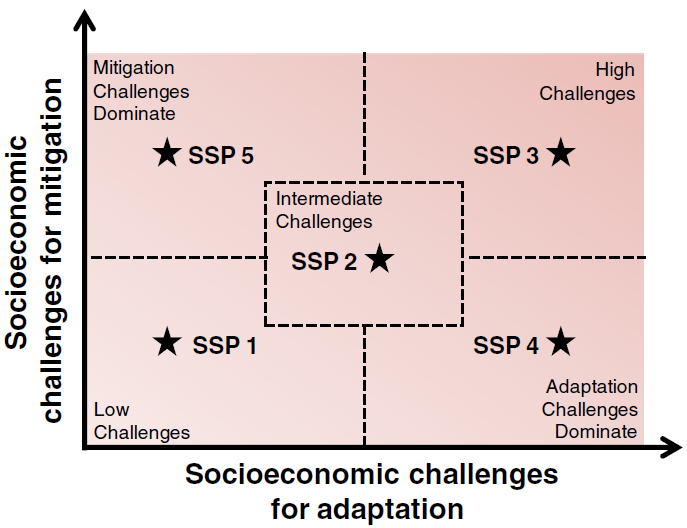
\includegraphics[width=.6\textwidth]{Pictures/SSPAxis}
	\caption{Five different future scenarios based on how clima change could affect society. Source: \citet{ConceptSSP}}
	\label{SSPAxis}
\end{figure}

The geosimulation has been run for five different future scenarios called the Shared Socioeconomic Pathways (SSPs). The different scenarios are based on different ways, climate change could affect society. As illustrated in figure \ref{SSPAxis} the five scenarios are based on two axes: socio-economic challenges for mitigation and for adaptation of climate change impacts. 
“Socio-economic” is referring to a large array of societal and socioecological systems. Covering aspects of a political, social, demographic, cultural, lifestyle, institutional, economic, and technological nature and condition of ecosystems. 
The horizontal axis is environmental or societal conditions, which would make adapting to climate change more difficult. This includes climate hazards (temperature and precipitation changes, sea level rise and extreme weather phenomena) and what and whom these hazards will affect.
\citep{ConceptSSP}
The vertical axis is factors, which in absence of climate policy would increase the amount of emissions of greenhouse gasses and factors reducing the society’s capacity to reduce those emissions. Examples of factors reducing society’s capacity is inadequate technologies and insufficient resources to support mitigation policies. The increase in greenhouse gasses could for example be a result of population and economic growth.
\citep{SSP}

\begin{table}[htbp]
	\centering
	\begin{tabular}{l}
		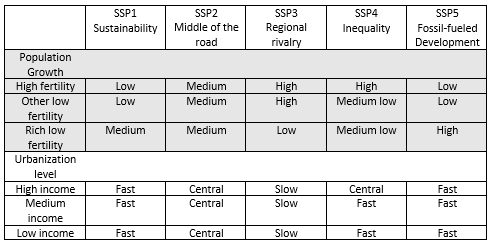
\includegraphics[width=0.8\textwidth]{Pictures/SSPTable}
	\end{tabular}
	\caption{Population growth and urbanization for each of the Shared Socioeconomic Pathways (SSP). Source: \citet{WhyDetailedPop}}
	\label{SSPTable}
\end{table}

How the population growth and the urbanization levels will be in the different scenarios can be seen in table \ref{SSPTable}. The population growth values are based on current income and fertility condition. The urbanization predictions are based on the current income. The Rich low fertility group has been defined as members of the Organisation for Economic Co-operation and Development.


\section{Technical details about the case data}\label{caseDataTech}

Table \ref{tabTech} is highlighting some technical specifications of the dataset, which will be important for the development. The technical details have been acquired using GDAL's raster information program, gdalinfo. GDAL is further described in section \ref{Librarygdal}.

\begin{table}[h]%You have to add this h yourself
	\centering
\begin{tabular}{|c|c|c|}
	\hline 
	\multicolumn{3}{|c|}{Technical information} \\ 
	\hline 
	Attribute & Value & Further explanation \\ 
	\hline 
	NoData value & -2147483648 &  \\ 
	\hline 
	Bit depth & 32 &  Section \ref{BitDepth}\\ 
	\hline 
	Projection & EPSG: 4326 &  Section \ref{ProjectionTheory}\\ 
	\hline 
	Projection unit & Degree &   \\ 
	\hline 
\end{tabular}
\caption{Technical attributes of the case data}
 \label{tabTech}
\end{table}

Some of these concepts will be explained in upcoming sections, but the NoData value will be explained here. A raster file has values for every pixel. If no data is available for a pixel, then the pixel gets assigned the NoData value. \citep{ArcMapOnNoData}

If the value was set to 0 it would be impossible to determine if an area had nobody living in it or if no data was available. That is the reason for the NoData value is set to a negative value, since the population density never can be negative.

